\chapter{生成式AI是什麼? (李弘毅生成式AI導論)}
\section{定義}
生成式人工智慧(Generative AI)是要讓機器產生複雜到無法窮舉且有結構的東西,例如文章、圖片、聲音,和分類(Classification)不同,選項有限的情況就不能稱為生成式AI。
\subsection{機器學習}
機器學習是指讓機器從資料中找到函式,
有上萬個未知參數的函式稱之為模型。
\subsubsection{訓練traning}
機器學習的學習指的就是把模型中上萬個參數找出來的過程,也稱為訓練。
\subsubsection{推論inference}
給訓練完的模型資料看他出來的結果會是什麼,這叫做測試,也叫做推論。

\subsection{深度學習}
深度學習(Deep Learning)是一種機器學習技術。把有大量參數的函式表示成一個類神經網路(Neural Network)再解出參數,就稱為深度學習。\\
今日的生成式人工智慧多以深度學習技術達成。

\begin{figure}[htbp!]
    \centering
    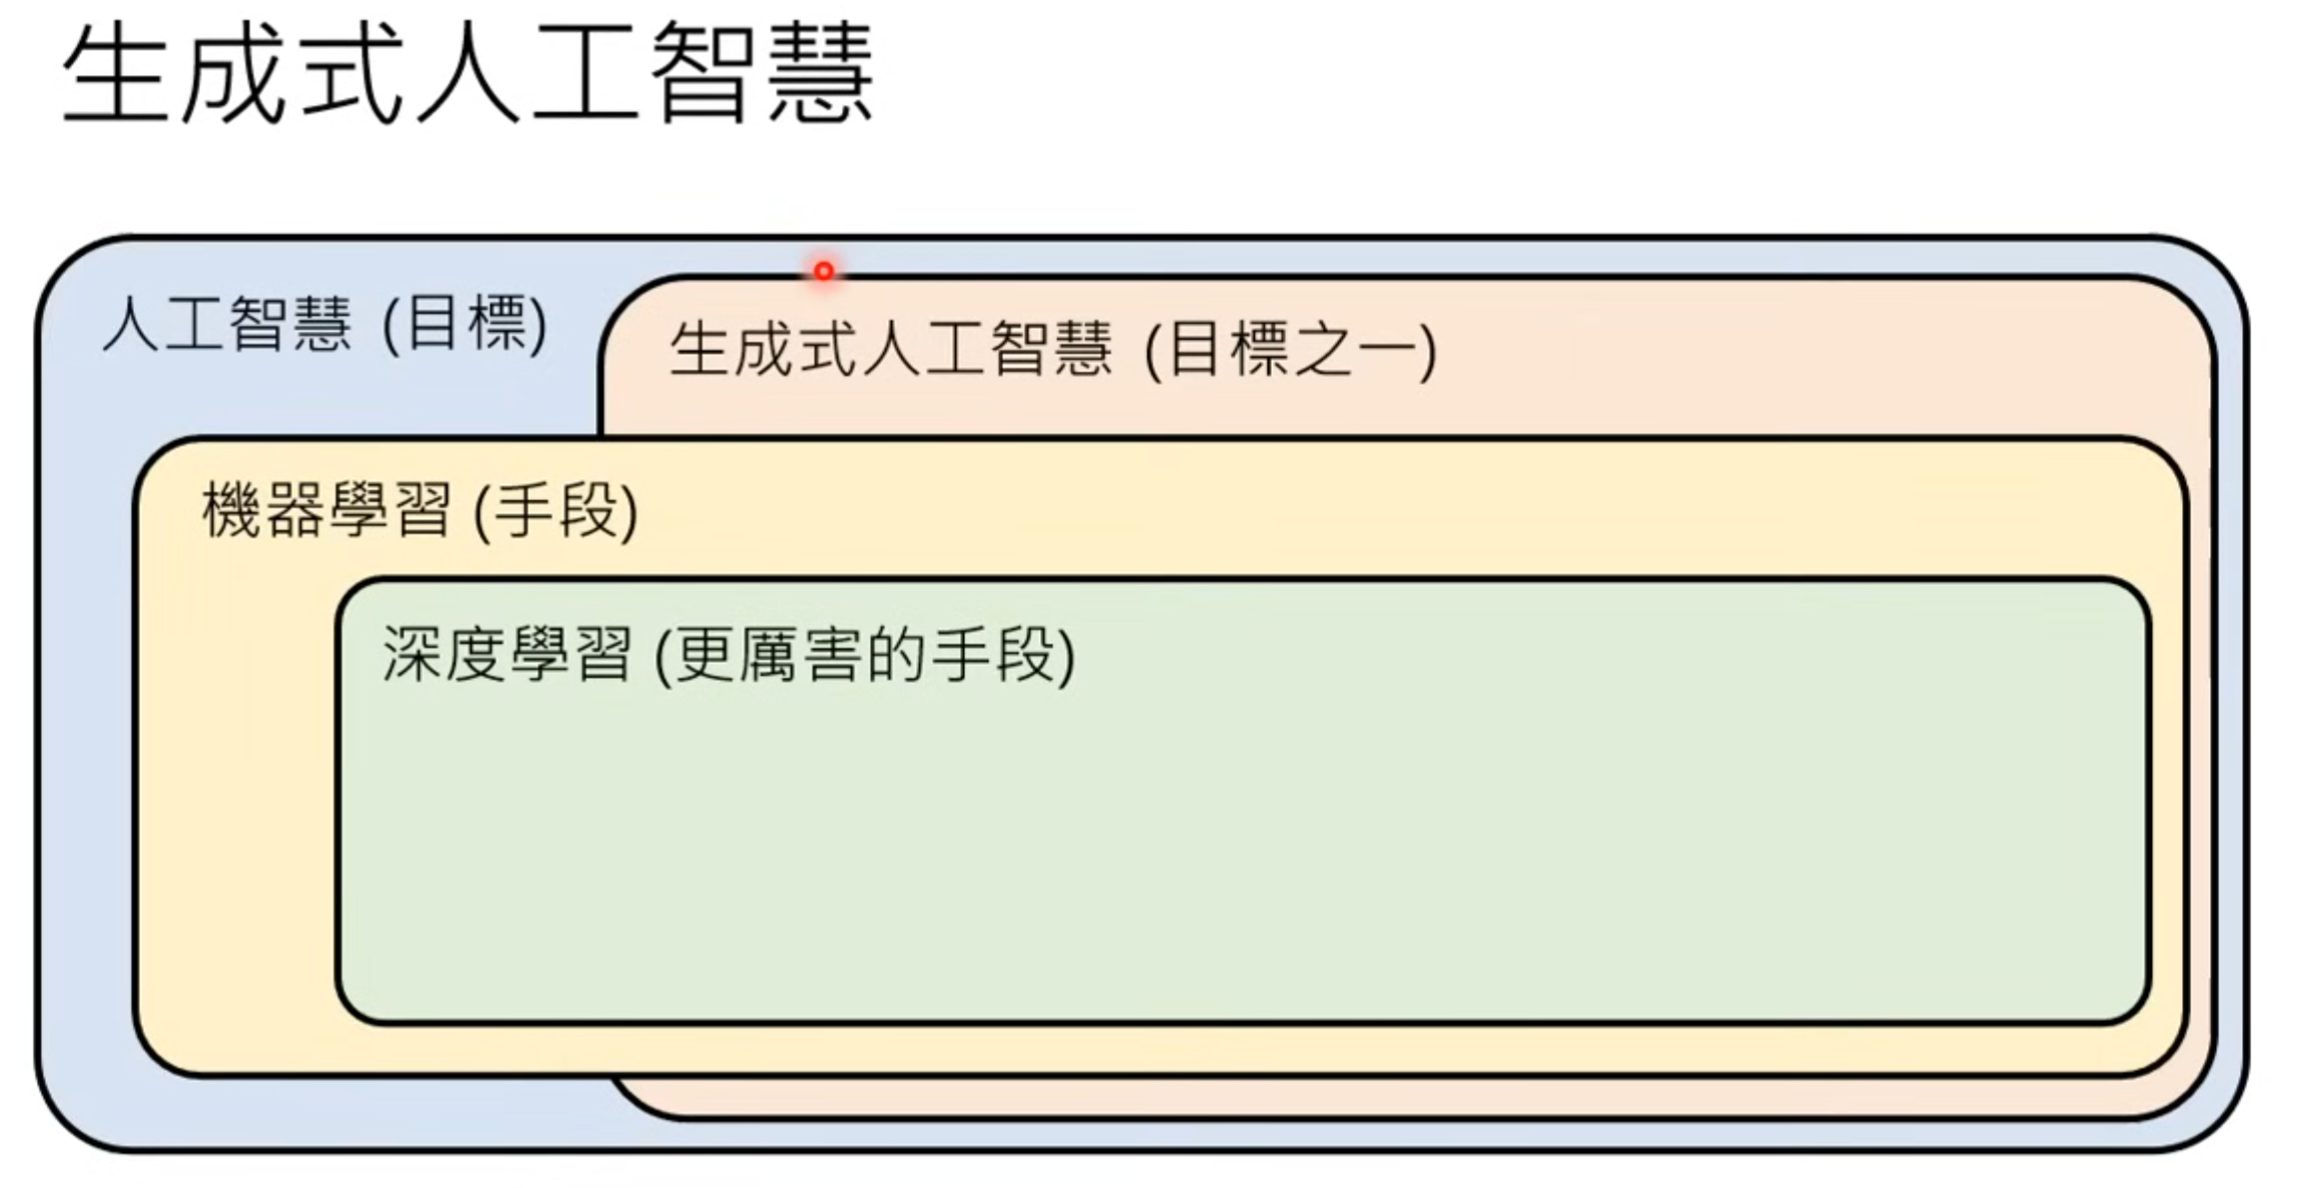
\includegraphics[width=0.5\linewidth]{images/w4/GAI.png}
    \caption{生成式AI關係圖}
    \label{fig:GAI}
\end{figure}

\section{ChatGPT}
ChatGPT可以想成是一個有上一個參數的模型。它的模型名稱叫做Transformer。
\begin{figure}[htbp!]
    \centering
    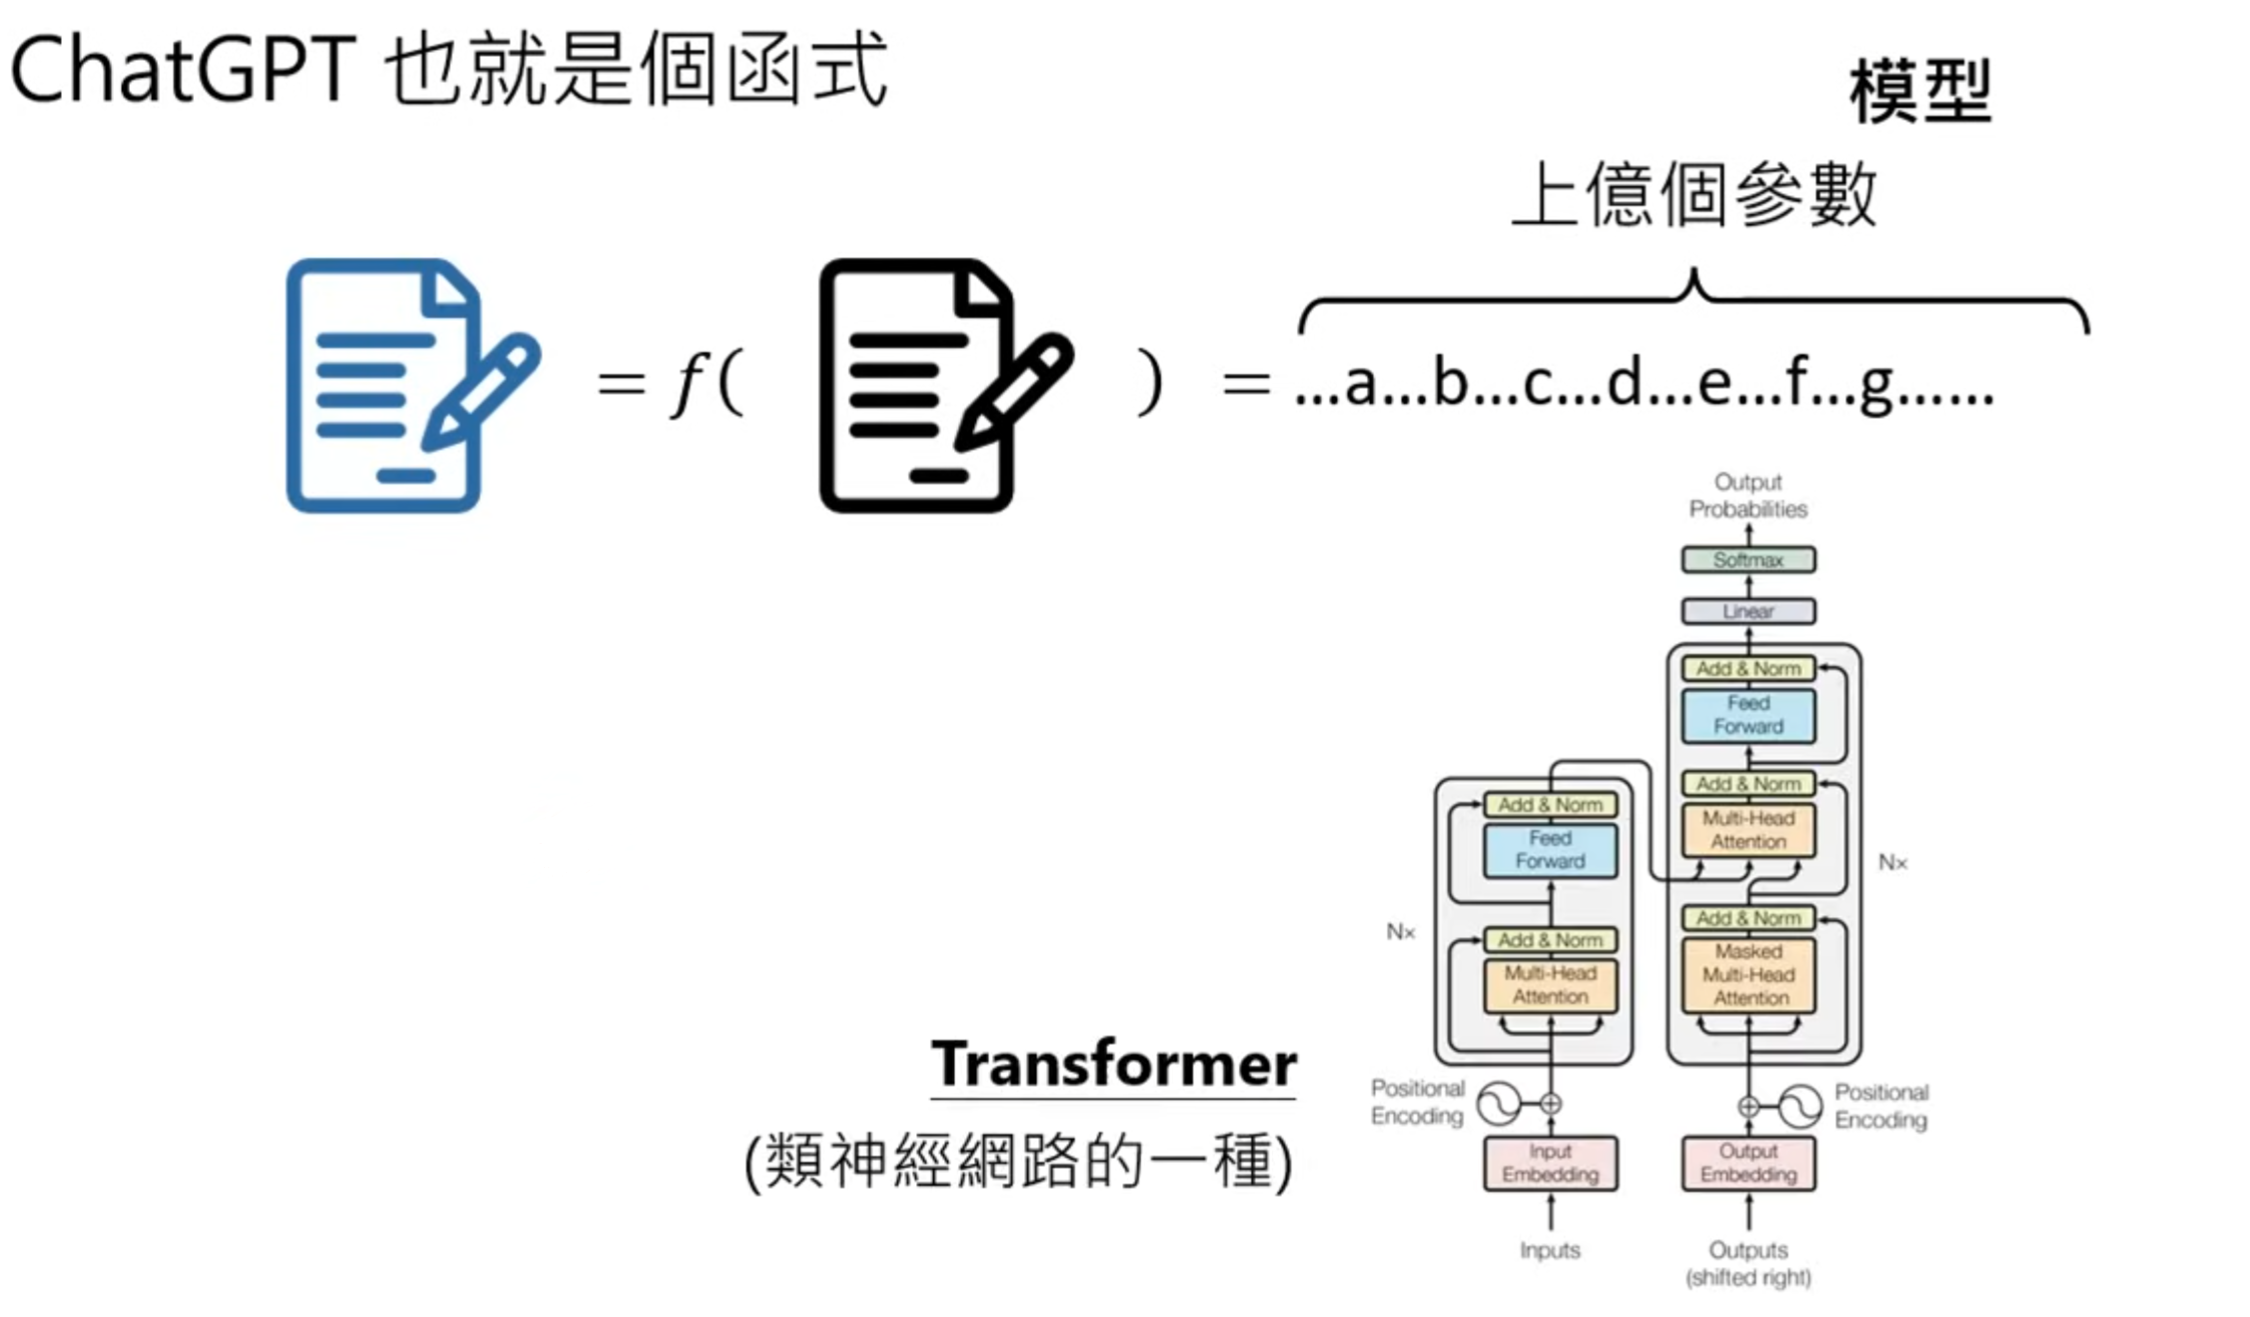
\includegraphics[width=0.6\linewidth]{images/w4/chatgptTransformer.png}
    \caption{ChatGPT和背後的模型}
    \label{fig:ChatGPT-Transformer}
\end{figure}

\subsection{文字接龍}
為了讓ChatGPT可以創造出訓練時沒有看過的文句,它所生成的答案可以拆解為一連串的文字接龍問題。\autoref{fig:language-model} 展示了文字接龍的模型,它被稱為語言模型。\\
語言模型可以把可能性無窮的問題換為一系列答案有限的分類問題。
\vfill
\begin{figure}[htbp!]
    \centering
    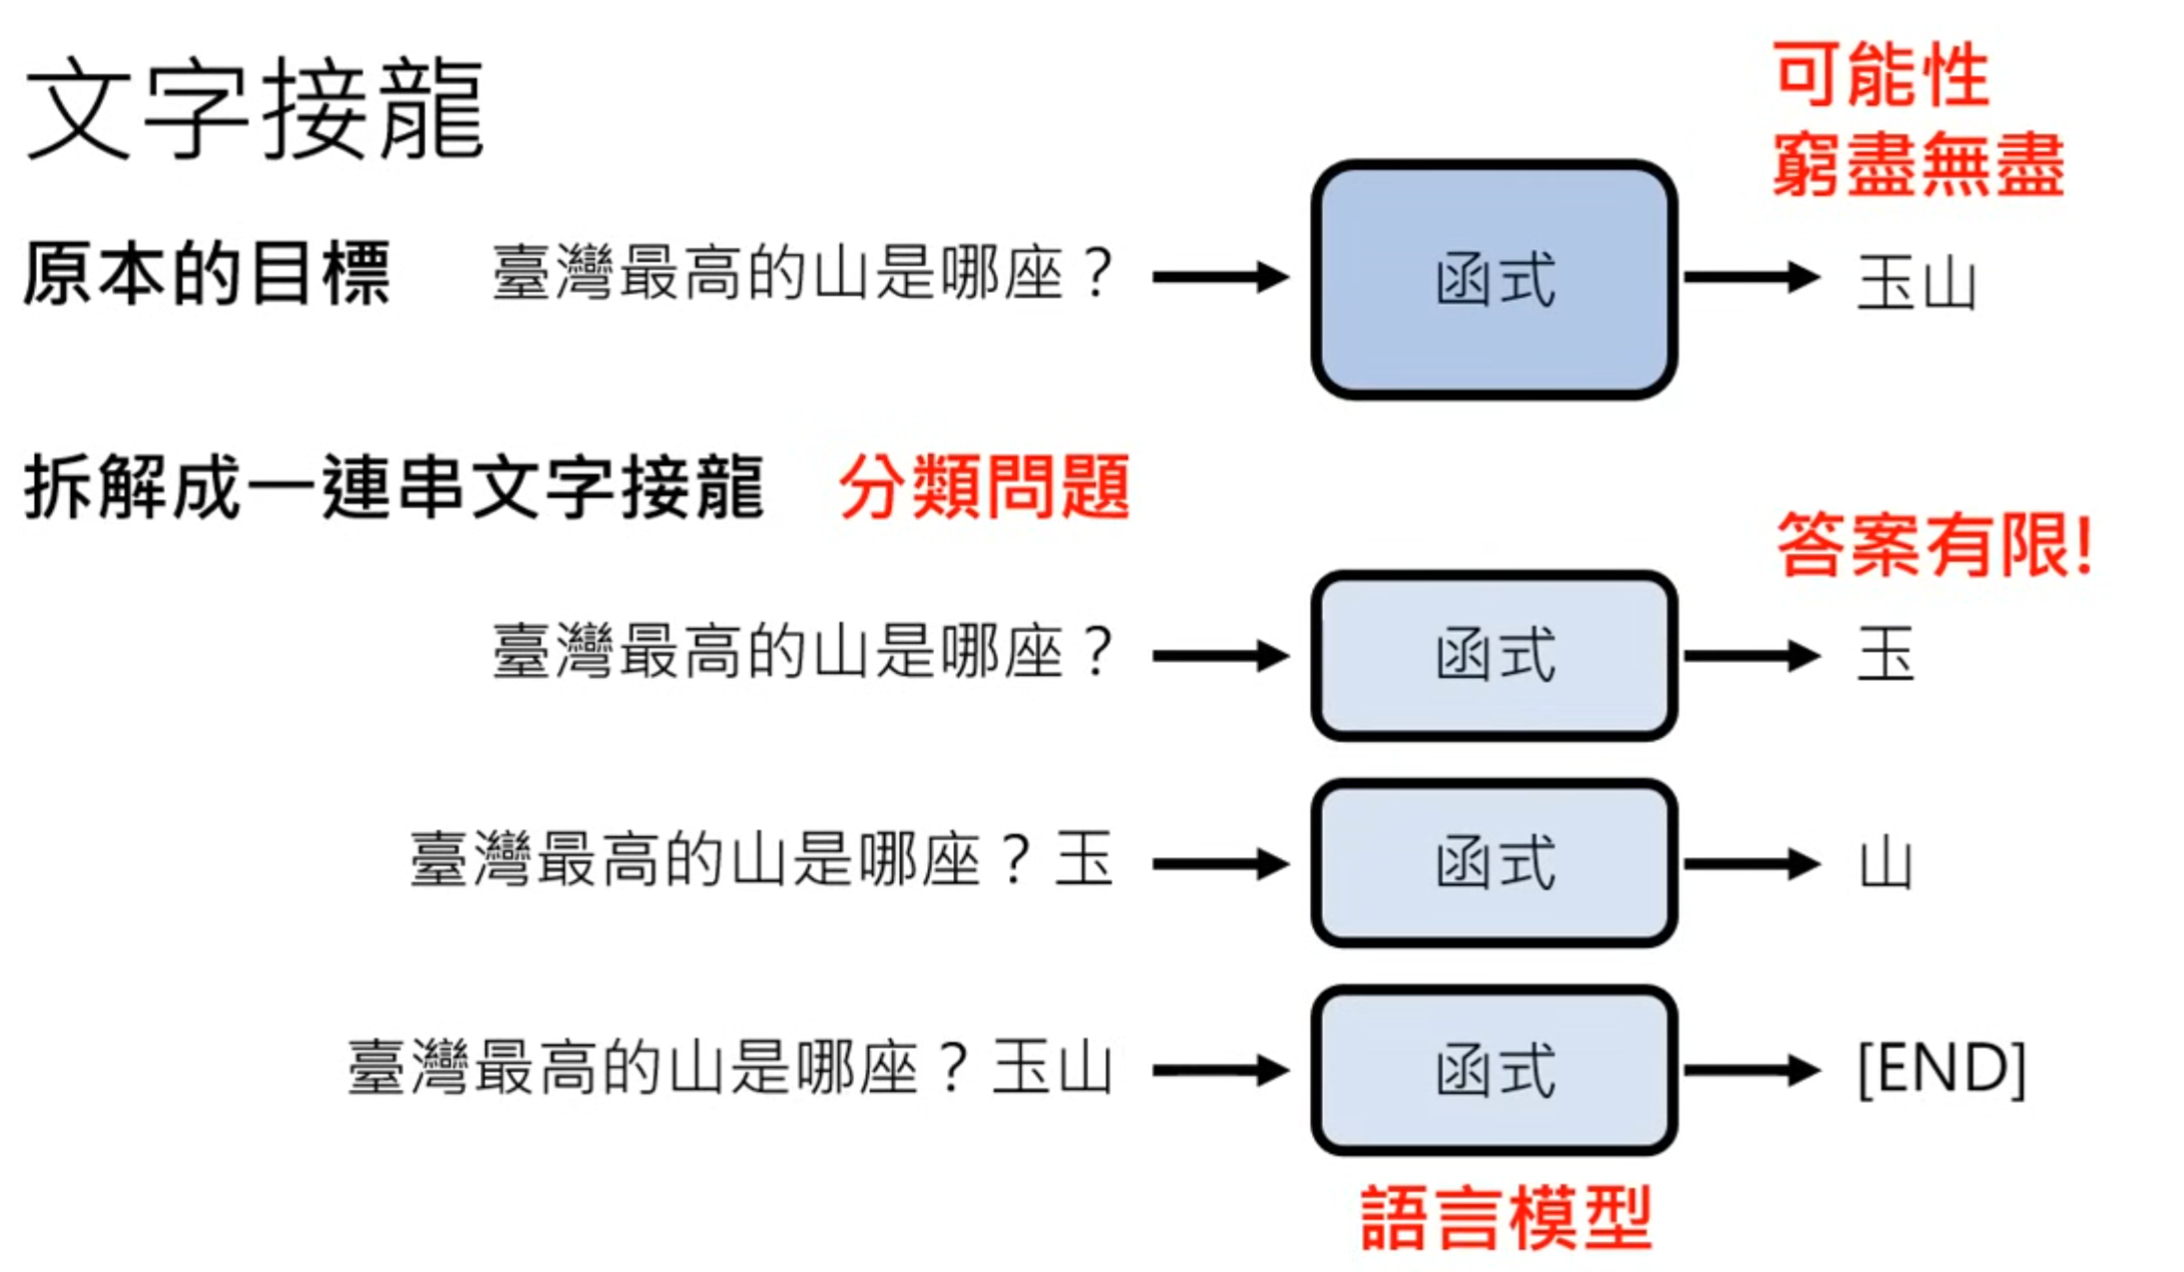
\includegraphics[width=0.6\linewidth]{images/w4/language-model.png}
    \caption{語言模型}
    \label{fig:language-model}
\end{figure}
\vfill
\newpage

\subsection{生成策略}
文章是由一序列的文字所組成,圖片是由像素所組成。它們都使把複雜的物件拆解後再依照某種順序把小單位生成出來,這種策略叫做Autoregressive Generation。

\begin{figure}[htbp!]
    \centering
    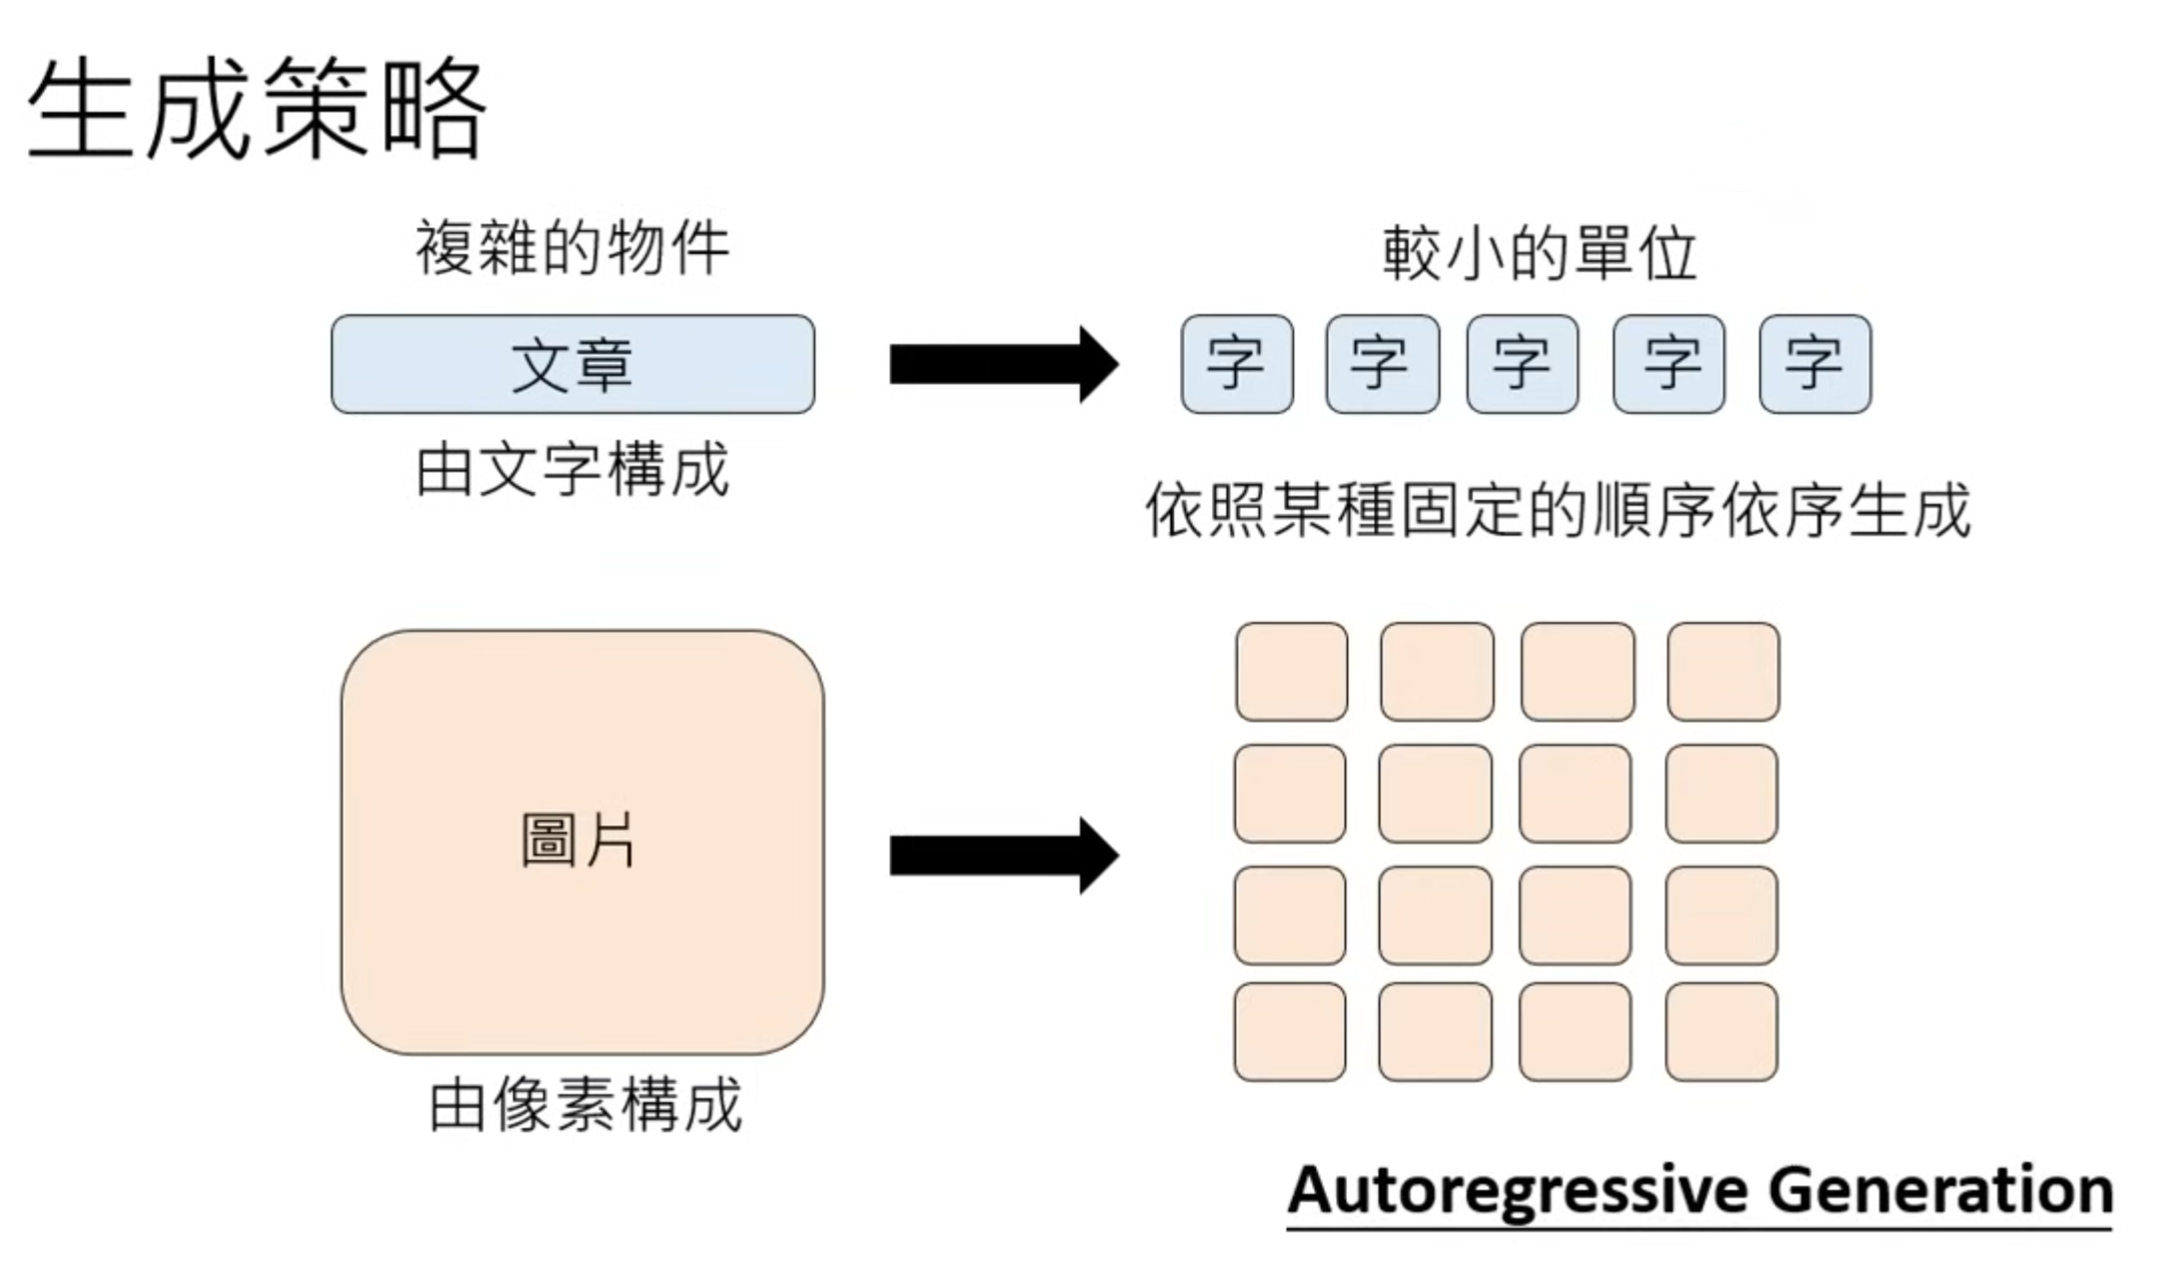
\includegraphics[width=0.6\linewidth]{images/w4/autoregressive-generation.png}
    \caption{生成策略示意圖}
    \label{fig:Autoregressive-Generation}
\end{figure}

\section{生成式AI知識圖}
\knowledgeGraph{images/w4/w4_taide.png}{生成式AI-TAIDE}{fig:GAI-TAIDE}{7.5}{\item 重要知識點都有列出來,能很好的理解中文
\item 知識圖結構簡單明瞭
}{\item 生成式人工智慧翻譯成"產生性人工智慧"
}{0.3}

\knowledgeGraph{images/w4/w4_zephyr.png}{生成式AI-Zephyr}{fig:GAI-Zephyr}{7}{\item 重要知識點都有列出來
\item 知識圖結構簡單明瞭
}{\item 有幾個有關聯性的節點沒有連接
}{0.3}

\knowledgeGraph{images/w4/w4_llama3.png}{生成式AI-Llama3}{fig:GAI-Llama3}{8.5}{\item 內容最為豐富
\item 有將語言模型和生成式人工智慧的技術連接到ChatGPT節點
}{\item 有一個意義不明的"投訴"節點
}{0.3}
\newpage


